\documentclass{article}

\usepackage{amsmath,graphicx,parskip}
\usepackage{fancyhdr}
\pagestyle{fancy}
\lhead{Samuel Huberman}
\chead{ECE1336:A8}
\rhead{999157923}

\newcommand{\unit}[1]{\ensuremath{\, \mathrm{#1}}}
\numberwithin{equation}{section}

\begin{document}

\section*{Problem 1}
The crystal momentum is defined as $\hbar k$, where $k$ is a real-valued wavevector determined by the solution of the one-electron Schrodinger equation in a periodic potential under appropriate boundary conditions (as was first done by Kronig and Penney). If energy is a parabolic function of $k$, the crystal momentum corresponds to the free particle momentum with a given effective mass.

\section*{Problem 2}
\begin{itemize}
\item a. Effective mass attempts to include the contribution of a periodic potential experienced by an electron and thereby provide a comparable picture with of free-electron. An electron in a periodic potential can be interpreted to be ``carrying around" the extra energy of this potential.
\begin{align*}
	m* &= \frac{\hbar^2}{d^2\epsilon/dk^2}
\end{align*}  
\item b. The dashed line has a smaller effective mass (larger curvature) than that of the solid line (smaller curvature). 
\item c. The effective mass as defined, affects the curvature of the E-k curve. The density of states describes the number of available states around an infinitesimal portion of energy. If we split the E-k curve into parcels of $\delta E$, we observe that a band with a larger curvature, corresponding to a smaller effective mass, has fewer states within this region $\delta E$. Qualitatively speaking, we can say the a larger effective mass corresponds to a greater density of states in a band with the vice versa being equally true.
\end{itemize}

\section*{Problem 3}
\begin{itemize}
\item a. See plot. 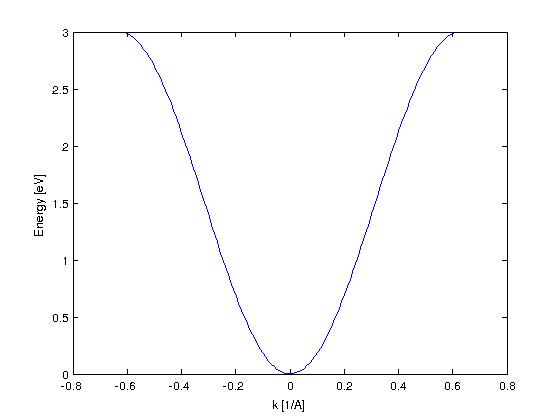
\includegraphics[scale=0.5]{A8q3.jpg}
\item b.
\begin{align*}
	m* &= \frac{\hbar^2}{d^2E/dk^2}\\
        \frac{d^2E}{dk^2}&=a^2E_0\cos(ka)
\end{align*}
For $k=0$:
\begin{align*}
	m* &= \frac{\hbar^2}{a^2E_0}\\
           & =1.85E-31 [kg]
\end{align*}
For $k=\pi/a$:
\begin{align*}
	m* &= \frac{\hbar^2}{-a^2E_0}\\
           & =-1.85E-31 [kg]
\end{align*}
\item c. Negative effective mass corresponds to the presence of vacant state, known as a hole.
\end{itemize}

\end{document}

